\chapter{Properties of Topological Spaces}

\section*{3.6.2.1. Hausdorff Property}

Definition 3.7 [First Separation Axiom] A topological space \(X\) satisfies the first separation axiom if for any two distinct points \(x \neq  y \in  X\) , there exists open \(U \ni  x\) but not including \(y\) .

Proposition 3.11 A topological space \(X\) has first separation property if and only if for \(\forall x \in  X,\{ x\}\) is closed in \(X\) .

Proof. Sufficiency. Suppose that \(x \neq  y\) , then construct \(U \mathrel{\text{ := }} X \smallsetminus  \{ y\}\) , which is a open set that contains \(x\) but not includes \(y\) .

Necessity. Take any \(x \in  X\) , then for \(\forall y \neq  x\) , there exists \(y \in  {U}_{y}\) that is open and \(x \notin  {U}_{y}\) . Thus

\[
\{ y\}  \subseteq  {U}_{y} \subseteq  X \smallsetminus  \{ x\}
\]

which implies

\[
\mathop{\bigcup }\limits_{{y \in  X \smallsetminus  \{ x\} }}\{ y\}  \subseteq  \mathop{\bigcup }\limits_{{y \in  X \smallsetminus  \{ x\} }}{U}_{y} \subseteq  X \smallsetminus  \{ x\}
\]

i.e., \(X \smallsetminus  \{ x\}  = \mathop{\bigcup }\limits_{{y \in  X\smallsetminus \{ x\} }}{U}_{y}\) is open in \(X\) , i.e., \(\{ x\}\) is closed in \(X\) .

Definition 3.8 [Second separation Axiom] A topological space satisfies the second separation axiom (or \(X\) is Hausdorff) if for all \(x \neq  y\) in \(X\) , there exists open sets \(U,V\) such that

\[
x \in  U,\;y \in  V,\;U \cap  V = \varnothing
\]

\begin{itemize}
\item Example 3.13 All metrizable topological spaces are Hausdorff.
\end{itemize}

Suppose \(d\left( {x,y}\right)  = r > 0\) , then take \({B}_{r/2}\left( x\right)\) and \({B}_{r/2}\left( y\right)\)

\begin{itemize}
\item Example 3.14 Note that a topological space that is first separable may not necessarily be second separable:
\end{itemize}

Consider \({\mathcal{T}}_{\text{ co-finite }}\) , then \(X\) is first separable but not Hausdorff:

Suppose on the contrary that for given \(x \neq  y\) , there exists open sets \(U,V\) such that \(x \in  U,y \in  V\) , and

\[
U \cap  V = \varnothing  \Rightarrow  X = X \smallsetminus  \left( {U \cap  V}\right)  = \left( {X \smallsetminus  U}\right)  \cup  \left( {X \smallsetminus  V}\right) ,
\]

implying that the union of two finite sets equals \(X\) , which is infinite, which is a contradiction.

\section*{4.3. Monday for MAT4002}

There will be a quiz next Monday. The scope is everything before CNY holiday. There will be one question with four parts for 40 minutes.

\section*{4.3.1. Hausdorffness}

Reviewing. A topological space(X, T)is said to be Hausdorff (or satisfy the second separtion property), if given any distinct points \(x,y \in  X\) , there exist disjoint open sets \(U,V\) such that \(U \ni  x\) and \(V \ni  y\) .

Proposition 4.5 If the topological space(X, T)is Hausdorff, then all sequences \(\left\{  {x}_{n}\right\}\) in \(X\) has at most one limit.

Proof. Suppose on the contrary that

\[
\left\{  {x}_{n}\right\}   \rightarrow  a,\;\left\{  {x}_{n}\right\}   \rightarrow  b\text{ , with }a \neq  b
\]

By separation property, there exists \(U,V \in  \mathcal{T}\) and \(U \cap  V = \varnothing\) such that \(U \ni  a\) and \(V \ni  b\) .

By tie openness of \(U\) , there exists \(N\) such that \(\left\{  {{x}_{N},{x}_{N + 1},\ldots }\right\}   \subseteq  U\) , since \(\left\{  {x}_{n}\right\}   \rightarrow  a \in  U\) . Similarly, there exists \(M\) such that \(\left\{  {{x}_{M},{x}_{M + 1},\ldots }\right\}   \subseteq  V\) . Take \(K = \max \{ M,N\}  + 1\) , then \(\varnothing  \neq  U \cap  V \ni  {x}_{K}\) , which is a contradiction.

Proposition 4.6 Let \(X,Y\) be Hausdorff spaces. Then \(X \times  Y\) is Hausdorff with product topology.

Proof. Suppose that \(\left( {{x}_{1},{y}_{1}}\right)  \neq  \left( {{x}_{2},{y}_{2}}\right)\) in \(X \times  Y\) . Then \({x}_{1} \neq  {x}_{2}\) or \({y}_{1} \neq  {y}_{2}\) . w.l.o.g., assume that \({x}_{1} \neq  {x}_{2}\) , then there exists \(U,V\) open in \(X\) such that \({x}_{1} \in  U,{x}_{2} \in  V\) with \(U \cap  V = \varnothing\) .

Therefore, we imply \(\left( {U \times  Y}\right) ,\left( {V \times  Y}\right)  \in  {\mathcal{T}}_{X \times  Y}\) , and

\[
\left( {U \times  Y}\right)  \cap  \left( {V \times  Y}\right)  = \left( {U \cap  V}\right)  \cap  Y = \varnothing
\]

with \(\left( {{x}_{1},{y}_{1}}\right)  \in  U \times  Y,\left( {{x}_{2},{y}_{2}}\right)  \in  V \times  Y\) , i.e., \(X \times  Y\) is Hausdorff with product topology.

The same argument applies if the second separation property is replaced by first separation property.

Proposition 4.7 If \(f : X \rightarrow  Y\) is an injective continuous mapping, then \(Y\) is Hausdorff implies \(X\) is Hausdorff.

Proof. Suppose that \(Y\) satisfies the second separation property. For given \(a \neq  b\) in \(X\) , we imply \(f\left( a\right)  \neq  f\left( b\right)\) in \(Y\) . Therefore, there exists \(U \ni  f\left( a\right) ,V \ni  f\left( b\right)\) with \(U \cap  V = \varnothing\) . It follows that

\[
a \in  {f}^{-1}\left( U\right) ,b \in  {f}^{-1}\left( V\right) ,\;{f}^{-1}\left( U\right)  \cap  {f}^{-1}\left( V\right)  = {f}^{-1}\left( {U \cap  V}\right)  = \varnothing ,
\]

i.e., \(X\) is Hausdorff.

Corollary 4.1 If \(f : X \rightarrow  Y\) is homeomorphic, then \(X\) is Hausdorff iff \(Y\) is Hausdorff, i.e., Hausdorffness is a topological property (i.e., a property that is preserved under homeomorphism).

\section*{4.3.2. Connectedness}

Definition 4.4 [Connected] The topological space(X, T)is disconnected if there are open \(U,V \in  \mathcal{T}\) such that

\[
U \neq  \varnothing ,V \neq  \varnothing ,\;U \cap  V = \varnothing ,\;U \cup  V = X. \tag{4.4}
\]

If no such \(U,V \in  \mathcal{T}\) exist, then \(X\) is connected.

Proposition 4.8 Let(X, T)be topological spaces. TFAE (i.e., the followings are equivalent):

1. \(X\) is connected

2. The only subset of \(X\) which are both open and closed are \(\varnothing\) and \(X\)

3. Any continuous function \(f : X \rightarrow  \{ 0,1\}\) ( \(\{ 0,1\}\) is equipped with discrete topology) is a constant function.

Proof. (1) implies (2): Suppose that \(U \subseteq  X\) is both open and closed. Then \(U,X \smallsetminus  U\) are both open and disjoint, and \(U \cup  \left( {X \smallsetminus  U}\right)  = X\) . By connnectedness, either \(U = \varnothing\) or \(X \smallsetminus  U = \varnothing\) . Therefore, \(U = \varnothing\) or \(X\) .

(2) implies (3): Note that \(U = {f}^{-1}\left( {\{ 0\} }\right)\) and \(V = {f}^{-1}\left( {\{ 1\} }\right)\) are open disjoint sets in \(X\) satisfying \(U \cup  V = X\) . By the connectedness of \(X\) , either \(\left( {U,V}\right)  = \left( {X,\varnothing }\right)\) or \(\left( {V,U}\right)  = \left( {\varnothing ,X}\right)\) . In either case, we imply \(f\) is a constant function.

(3) implies (2): Suppose that \(U \subseteq  X\) is both open and closed. Construct the mapping

\[
f\left( x\right)  = \left\{  \begin{array}{ll} 0, & x \in  U \\  1, & x \in  X \smallsetminus  U \end{array}\right.
\]

It’s clear that \(f\) is continuous, and therefore \(f\left( x\right)  = 0\) or 1 . Therefore \(U = \varnothing\) or \(X\) .

(2) implies (1): Suppose on the contrary that there exists open \(U,V\) such that (4.4) holds. By (4.4), we imply \(U = X \smallsetminus  V\) is closed as well. Since \(U \neq  \varnothing\) and \(U = \varnothing\) or \(X\) , we imply \(U = X\) , which implies \(V = \varnothing\) , which is a contradiction.

\section*{Corollary 4.2 The interval \(\left\lbrack  {a,b}\right\rbrack   \subseteq  \mathbb{R}\) is connnected}

Proof. Suppose on the contrary that there exists continuous function \(f : \left\lbrack  {a,b}\right\rbrack   \rightarrow  \{ 0,1\}\) that takes 2 values. Construct the mapping \(\widetilde{f} : \left\lbrack  {a,b}\right\rbrack   \rightarrow  \mathbb{R}\)

\[
\widetilde{f} : \left\lbrack  {a,b}\right\rbrack  \overset{f}{ \rightarrow  }\{ 0,1\} \overset{i}{ \rightarrow  }\mathbb{R}
\]

\[
\text{ with }\widetilde{f} = i \circ  f\text{ . }
\]

Note that \(\{ 0,1\}  \subseteq  \mathbb{R}\) denotes the subspace topology, we imply the inclusion mapping \(i : \{ 0,1\}  \rightarrow  \mathbb{R}\) with \(s \mapsto  s\) is continuous. The composition of continuous mappings is continuous as well, i.e., \(\widetilde{f}\) is continuous.

Since the function \(f\) can take two values, there exists \(p,q \in  \left\lbrack  {a,b}\right\rbrack\) such that \(\widetilde{f}\left( p\right)  =\)  \(i \circ  f\left( p\right)  = 0\) and \(\widetilde{f}\left( q\right)  = i \circ  f\left( q\right)  = 1\) . By intermediate value theorem, there exists \(r \in  \left\lbrack  {a,b}\right\rbrack\) such that \(\widetilde{f}\left( r\right)  = i \circ  f\left( r\right)  = 1/2\) , which implies \(f\left( r\right)  = \frac{1}{2}\) , which is a contradiction.

Definition 4.5 [Connected subset] A non-empty subset \(S \subseteq  X\) is connected if \(S\) with the subspace topology is connected

Equivalently, \(S \subseteq  X\) is connected if, whenever \(U,V\) are open in \(X\) such that \(S \subseteq  U \cup  V\) , and \(\left( {U \cap  V}\right)  \cap  S = \varnothing\) , one can imply either \(U \cap  S = \varnothing\) or \(V \cap  S = \varnothing\) .

Proposition 4.9 If \(f : X \rightarrow  Y\) is continuous mapping, and the subset \(A \subseteq  X\) is connected, then \(f\left( A\right)\) is connected. In other words, the continuous image of a connected set is connected.

Proof. Suppose that \(U,V \subseteq  Y\) is open such that

\[
f\left( A\right)  \subseteq  U \cup  V,\;\left( {U \cap  V}\right)  \cap  f\left( A\right)  = \varnothing .
\]

Therefore we imply

\[
A \subseteq  {f}^{-1}\left( U\right)  \cup  {f}^{-1}\left( V\right) ,\;\left( {{f}^{-1}\left( U\right)  \cap  A}\right)  \cap  \left( {{f}^{-1}\left( V\right)  \cap  A}\right)  = \varnothing
\]

By connectedness of \(A\) , either \({f}^{-1}\left( U\right)  \cap  A = \varnothing\) or \({f}^{-1}\left( V\right)  \cap  A = \varnothing\) . Therefore, \(f\left( A\right)  \cap  U = \varnothing\) or \(f\left( A\right)  \cap  V = \varnothing\) , i.e., \(f\left( A\right)\) is connected.

Proposition 4.10 If \({\left\{  {A}_{i}\right\}  }_{i \in  I}\) are connnected and \({A}_{i} \cap  {A}_{j} \neq  \varnothing\) for \(\forall i,j \in  I\) , then the set \(\mathop{\bigcup }\limits_{{i \in  I}}{A}_{i}\) is connected.

Proof. Suppose the function \(f : { \cup  }_{i \in  I}{A}_{i} \rightarrow  \{ 0,1\}\) is a continuous map. Then we imply that its restriction \({\left. f\right| }_{{A}_{i}} = f \circ  i : {A}_{i} \rightarrow  \{ 0,1\}\) is continuous for all \(i \in  I\) . Thus \({\left. f\right| }_{{A}_{i}}\) is a constant for all \(i \in  I\) . Due to the non-empty intersection of \({A}_{i},{A}_{j}\) for \(\forall i,j \in  I\) , we imply \(f\) is constant.

Proposition 4.11 If \(X,Y\) are connnected, then \(X \times  Y\) is connected using product topology.

Proof. It’s clear that \(X \times  \left\{  {y}_{0}\right\}\) is connected in \(X \times  Y\) for fixed \({y}_{0}\) ; and \(\left\{  {x}_{0}\right\}   \times  Y\) is connected for fixed \({x}_{0}\) .

Therefore, for fixed \({y}_{0} \in  Y\) , construct \(B = X \times  \left\{  {y}_{0}\right\}\) and \({C}_{x} = \{ x\}  \times  Y\) , which follows that

\[
B \cap  {C}_{x} = \left\{  \left( {x,{y}_{0}}\right) \right\}   \neq  \varnothing ,\forall x \in  X \Rightarrow  B \cup  \left\{  {\mathop{\bigcup }\limits_{{x \in  X}}{C}_{x}}\right\}   = X \times  Y\text{ is connected. }
\]

Definition 4.6 [Path Connectes] Let(X, T)be a topological space.

1. A path connecting 2 points \(x,y \in  X\) is a continuous function \(\tau  : \left\lbrack  {0,1}\right\rbrack   \rightarrow  X\) with \(\tau \left( 0\right)  = x,\tau \left( 1\right)  = y\) .

2. \(X\) is path-connected if any 2 points in \(X\) can be connected by a path.

3. The set \(A \subseteq  X\) is path-connected, if \(A\) sastisfies the condition using subspace topology.

Or equivalently, \(A\) is path-connected if for any 2 points in \(X\) , there exists a continuous \(t : \left\lbrack  {0,1}\right\rbrack   \rightarrow  X\) with \(t\left( x\right)  \in  A\) for any \(x\) , connecting the 2 points.

\section*{4.6. Wednesday for MAT4002}

There will be a quiz on Monday.

Reviewing.

\begin{itemize}
\item Connectedness / Path-Connectedness
\end{itemize}

\section*{4.6.1. Remark on Connectedness}

Proposition 4.14 All path connected spaces \(X\) are connected.

Proof. Fix any \(x \in  X\) , for all \(y \in  X\) , there exists a continuous mapping \({p}_{y} : \left\lbrack  {0,1}\right\rbrack   \rightarrow  X\) such that

\[
{p}_{y}\left( 0\right)  = x,\;{p}_{y}\left( 1\right)  = y.
\]

Consider \({C}_{y} = {p}_{y}\left( \left\lbrack  {0,1}\right\rbrack  \right)\) , which is connected, due to proposition (4.9).

Note that \({\left\{  {C}_{y}\right\}  }_{y \in  X}\) is a collection of connected sets, and for any \(y,{y}^{\prime } \in  X,{C}_{y} \cap  {C}_{{y}^{\prime }} \ni\)  \(\{ x\}\) is non-empty. Applying proposition (4.10), we imply \(X = { \cup  }_{y \in  X}{C}_{y}\) is connected.

\begin{itemize}
\item Example 4.5 1. Exercise: if \(A \subset  B \subset  \bar{A}\) , then \(A\) is connected implies \(B\) is connected. (Hint: \(U \cap  A = \varnothing\) implies \(U \cap  \bar{A} = \varnothing\) for all open sets \(U\) in \(X\) .)
\end{itemize}

Proof. Suppose \(B\) is not connected, i.e., for any open \(U,V\) such that \(B \subseteq  U \cup  V\) and \(\left( {U \cap  V}\right)  \cap  B = \varnothing\) , we imply \(U \cap  B \neq  \varnothing\) and \(V \cap  B \neq  \varnothing\) , and therefore

\[
U \cap  \bar{A} \neq  \varnothing ,\;V \cap  \bar{A} \neq  \varnothing
\]

which implies

\[
U \cap  A \neq  \varnothing ,\;V \cap  A \neq  \varnothing
\]

which contradicts to the connectedness of \(A\) .

2. The converse of proposition (4.14) may not be necessarily true. Consider the so-called Topologist's comb example:

\begin{center}
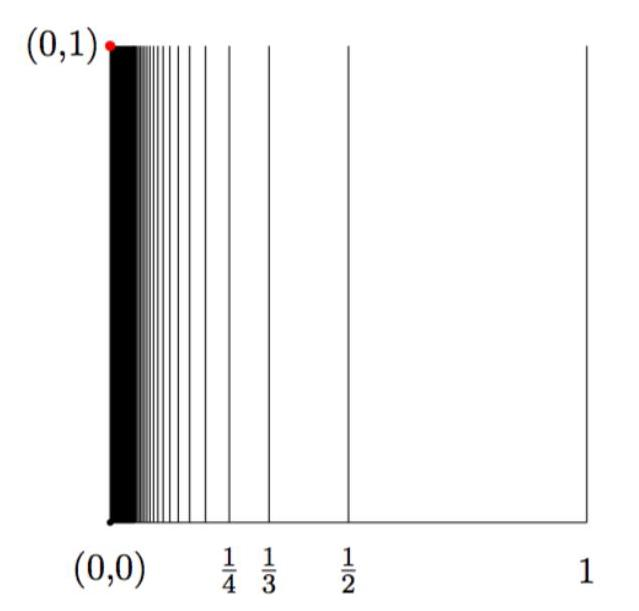
\includegraphics[max width=0.5\textwidth]{images/bo_d2bcsrref24c73avs720_52_671_318_639_611_0.jpg}
\end{center}
\hspace*{3em} 

Figure 4.1: Connected space \(X\) but not path-connected

Here we construct a connected space \(X \subseteq  {\mathbb{R}}^{2}\) but not path-connected shown in Fig (4.1), i.e., the union of the interval \(\left\lbrack  {0,1}\right\rbrack\) together with vertical line segments from \(\left( {1/n,0}\right)\) to \(\left( {1/n,1}\right)\) and the single point(0,1).

\[
X = \left( {\left\lbrack  {0,1}\right\rbrack  \times \{ 0\} }\right)  \cup  \mathop{\bigcup }\limits_{{n \geq  1}}\left( {\{ 1/n\}  \times  \left\lbrack  {0,1}\right\rbrack  }\right)  \cup  \left( {0,1}\right) .
\]

(a) Firstly, \(X\) is not path-connected. We show that there is no path in \(X\) links(0,1) to any other point, i.e., for continuous mapping \(p : \left\lbrack  {0,1}\right\rbrack   \rightarrow  X\) with \(p\left( 0\right)  = \left( {0,1}\right)\) , we may imply \(p\left( t\right)  = \left( {0,1}\right)\) for any \(t\) .

Define

\[
A = \{ t \in  \left\lbrack  {0,1}\right\rbrack   \mid  p\left( t\right)  = \left( {0,1}\right) \} .
\]

We claim that \(A = \left\lbrack  {0,1}\right\rbrack\) , i.e., suffices to show \(A\) is both open and closed in \(\left\lbrack  {0,1}\right\rbrack   :\)

i. The set \(A = {p}^{-1}\left( \left( {0,1}\right) \right)\) is nonempty and closed, since the pre-image of a closed set is closed as well.

ii. The set \(A\) is open: choose \({t}_{0} \in  A\) . By continuity of \(p\) , there exists \(\delta  > 0\) such that

\[
\parallel p\left( t\right)  - \left( {0,1}\right) \parallel  = \begin{Vmatrix}{p\left( t\right)  - p\left( {t}_{0}\right) }\end{Vmatrix} < \frac{1}{2},\;t \in  \left\lbrack  {0,1}\right\rbrack   \cap  \left( {{t}_{0} - \delta ,{t}_{0} + \delta }\right) .
\]

Since there is no point on the \(x\) -axis with the distance \(1/2\) to the point (0,1), we imply \(p\left( t\right)\) is not on the \(x\) -axis when \(t \in  \left\lbrack  {0,1}\right\rbrack   \cap  \left( {{t}_{0} - \delta ,{t}_{0} + \delta }\right)\) . Therefore, the \(x\) -coordinate of \(p\left( t\right)\) is either 0 or of the form \(1/n\) .

It suffices to show the open interval \(I \mathrel{\text{ := }} \left\lbrack  {0,1}\right\rbrack   \cap  \left( {{t}_{0} - \delta ,{t}_{0} + \delta }\right)\) is in \(A\) . Define the composite function \(f = x \circ  p : I \rightarrow  \mathbb{R}\) , where the mapping \(x : {\mathbb{R}}^{2} \rightarrow  \mathbb{R}\) is defined as \(\left( {a,b}\right)  \mapsto  a\) . Note that \(I\) is connected, we imply \(f\left( I\right)\) is connected, and \(f\left( I\right)\) belongs to \(\{ 0\}  \cup  \{ 1/n\}\) .

The only nonempty connected subset of \(\{ 0\}  \cup  \{ 1/n\}\) is a single point (left as exercise), and therefore \(f\left( I\right)\) is a single point. Since \(f\left( {t}_{0}\right)  = 0\) , we imply \(f\left( I\right)  = \{ 0\}\) , i.e., \(I \subseteq  A\) . Therefore \(A\) is open.

\section*{4.6.2. Compactness}

Compact set in \(X\) is used to generalize "closed and bounded" in \({\mathbb{R}}^{n}\) .

Definition 4.11 Let(X, T)be a topological space. A collection \(\mathcal{U} = \left\{  {{U}_{i} \mid  i \in  I}\right\}\) of open sets is an open cover of \(X\) if

\[
X = \mathop{\bigcup }\limits_{{i \in  I}}{U}_{i}
\]

A subcover of \(\mathcal{U}\) is a subfamily

\[
{\mathcal{U}}^{\prime } = \left\{  {{U}_{j} \mid  j \in  J}\right\}  ,\;J \subseteq  I
\]

such that \(\mathop{\bigcup }\limits_{{j \in  J}}{U}_{j} = X\) .

If \(J\) has finitely many elements, we say \({\mathcal{U}}^{\prime }\) is a finite subcover of \(X\) .

We say \(X\) is compact if any open cover of \(X\) has a finite subcover.

If \(A \subseteq  X\) has a subspace topology. then \(A\) is compact iff for any open collection of open sets (in \(X\) ) \(\left\{  {U}_{i}\right\}\) such that \(A \subseteq  \mathop{\bigcup }\limits_{{i \in  I}}{U}_{i}\) , there exists a fintie subcover \(A \subseteq  \mathop{\bigcup }\limits_{{k = 1}}^{n}{U}_{{i}_{k}}\) .

Proposition 4.15 Let \(X\) be a topological space. The followings are equivalent:

1. The space \(X\) is compact

2. If \(\left\{  {{V}_{i} \mid  i \in  I}\right\}\) is a collection of closed subsets in \(X\) such that

\[
\mathop{\bigcap }\limits_{{j \in  J}}{V}_{j} \neq  \varnothing ,\;\text{ for all finite }J \subseteq  I,
\]

then \({ \cap  }_{i \in  I}{V}_{i} \neq  \varnothing\) .

Compactness is an intrisical property, i.e., we do not need to worry about which underlying space for this definition.

\begin{itemize}
\item Example 4.6 1. \(X \subseteq  {\mathbb{R}}^{n}\) is compact iff \(X\) is closed and bounded. (Heine-Borel)
\end{itemize}

2. Let \(K \subseteq  {\mathbb{R}}^{n}\) be compact, then define the set

\(\mathcal{C}\left( K\right)  = \{\) all continuous mapping \(f : K \rightarrow  \mathbb{R}\}\)

Note that the \({d}_{\infty }\) metric associated with \(\mathcal{C}\left( K\right)\) , say \(\parallel f{\parallel }_{\infty } = \mathop{\sup }\limits_{{k \in  K}}f\left( k\right)\) , is well-defined.

Under the metric space \(\left( {\mathcal{C}\left( K\right) ,{d}_{\infty }}\right)\) , any \(\mathcal{J} \subseteq  \mathcal{C}\left( K\right)\) is compact, if and only if \(\mathcal{J}\) is

closed, bounded, and equi-continuous. (Aresul-Ascoli)

Therefore, we can see that the compactness is not equivalent to the closedness together with boundedness.

Proposition 4.16 Let \(X\) be a compact space, then all closed subset \(A \subseteq  X\) are compact.

Proof. Let \(\left\{  {{V}_{i} \mid  i \in  I}\right\}\) be a collection of closed subsets in \(A\) such that

\[
{ \cap  }_{j \in  J}{V}_{j} \neq  \varnothing ,\;\text{ for any finite }J \subseteq  I\text{ . }
\]

As \(A\) is closed in \(X\) , we imply \({V}_{j}\) is closed in \(X\) .

Due to the compactness of \(X\) and proposition (4.15), we imply

\[
{ \cap  }_{i \in  I}{V}_{i} \neq  \varnothing
\]

By the reverse direction of proposition (4.15), we imply \(A\) is compact.

Now consider the reverse direction of proposition (4.16), i.e., are all compact subsets \(K \subseteq  X\) closed in \(X\) ?

In general, the converse does not hold. Note that \(K = \{ x\}\) is compact for any topology \(X\) . However, there are some topologies such that \(\{ x\}\) is closed.

In order to obtain the converse of proposition (4.16), we need to obtain another

\section*{separation axiom:}

Proposition 4.17 Let \(X\) be Hausdorff, \(K \subseteq  X\) be compact, and \(x \in  X \smallsetminus  K\) . Then there exists open \(U,V \subseteq  X\) such that \(U \cap  V = \varnothing\) and

\[
U \cap  V = \varnothing ,\;K \subseteq  U,\;x \in  V.
\]

Proof. Let \(k \in  K\) , then by Hausdorffness, there exists open \({U}_{k} \ni  k,{V}_{k} \ni  x\) such that \({U}_{k} \cap  {V}_{k} = \varnothing\) . Therefore, \({\left\{  {U}_{k}\right\}  }_{k \in  K}\) forms an open cover of \(K\) . By compactness of \(K\) , \({\left\{  {U}_{{k}_{i}}\right\}  }_{i = 1}^{n}\) covers \(K\) . Constructing the set

\[
U \mathrel{\text{ := }} \mathop{\bigcup }\limits_{{i = 1}}^{n}{U}_{{k}_{i}},\;V = \mathop{\bigcap }\limits_{{i = 1}}^{n}{V}_{{k}_{i}}
\]

gives the desired result.

By making use of this separation axiom, we obtain the converse of proposition (4.16):

Corollary 4.3 All compact \(K\) in Hausdorff \(X\) is closed.

Proof. For \(\forall x \in  X \smallsetminus  K\) , by proposition (4.17) there exists open \(V\) such that \(x \in  V \subseteq  X \smallsetminus  K\) , and therefore \(X \smallsetminus  K\) is open.

\section*{5.3. Monday for MAT4002}

\section*{5.3.1. Continuous Functions on Compact Space}

Proposition 5.3 Let \(f : X \rightarrow  Y\) be continuous function on topological spaces, with \(A \subseteq  X\) compact. Then \(f\left( A\right)  \subseteq  Y\) is compact.

Proof. Let \(\left\{  {{U}_{i} \mid  i \in  I}\right\}\) be an open cover of \(f\left( A\right)\) , i.e.,

\[
f\left( A\right)  \subseteq  \mathop{\bigcup }\limits_{{i \in  I}}{U}_{i},\;{U}_{i} \in  {\mathcal{T}}_{Y}
\]

It follows that \(\left\{  {{f}^{-1}\left( {U}_{i}\right)  \mid  i \in  I}\right\}\) is an open cover of \(A\) :

\[
A \subseteq  {f}^{-1}\left( {\mathop{\bigcup }\limits_{{i \in  I}}{U}_{i}}\right)  = \mathop{\bigcup }\limits_{{i \in  I}}{f}^{-1}\left( {U}_{i}\right)
\]

By the compactness of \(A\) , there exists finite subcover of \(A\) :

\[
A \subseteq  \mathop{\bigcup }\limits_{{k = 1}}^{n}{f}^{-1}\left( {U}_{{i}_{k}}\right)
\]

which implies the constructed finite subcover of \(f\left( A\right)\) :

\[
f\left( A\right)  \subseteq  f\left( {{ \cup  }_{k = 1}^{n}{f}^{-1}\left( {U}_{{i}_{k}}\right) }\right)
\]

\[
= {\bigcup }_{k = 1}^{n}{U}_{{i}_{k}}
\]

lary 5.2 1. Suppose that \(X\) is compact, and the mapping \(f : X \rightarrow  \mathbb{R}\) is continuous, then \(f\left( X\right)\) is closed and bounded, i.e., there exists \(m,M \in  X\) such that

\[
f\left( m\right)  \leq  f\left( x\right)  \leq  f\left( M\right) ,\forall x \in  X.
\]

2. Suppose moreover that \(X\) is connected, then

\[
f\left( X\right)  = \left\lbrack  {f\left( m\right) ,f\left( M\right) }\right\rbrack  .
\]

Theorem 5.2 The space \(X,Y\) are compact iff \(X \times  Y\) is compact under product topology.

Proof. 1. Sufficiency: Given that \(X \times  Y\) is compact, consider the projection mapping (which is continuous):

\[
\left\{  \begin{array}{l} {P}_{X} : X \times  Y \rightarrow  X \\  {P}_{Y} : X \times  Y \rightarrow  Y \end{array}\right.
\]

By applying proposition (5.3), \({P}_{X}\left( {X \times  Y}\right)  = X,{P}_{Y}\left( {X \times  Y}\right)  = Y\) are both compact.

2. Necessity: Suppose that \({\left\{  {W}_{i}\right\}  }_{i \in  I}\) is an open cover of \(X \times  Y\) . Each open set \({W}_{i}\) can be written as:

\[
{W}_{i} = \mathop{\bigcup }\limits_{{j \in  {\mathcal{J}}_{i}}}{U}_{ij} \times  {V}_{ij},\;{U}_{ij} \in  {\mathcal{T}}_{X},{V}_{ij} \in  {\mathcal{T}}_{Y}.
\]

It follows that

\[
X \times  Y = \mathop{\bigcup }\limits_{{\left( {i,j}\right)  \in  K}}{U}_{ij} \times  {V}_{ij},\;K = \left\{  {\left( {i,j}\right)  \mid  i \in  I,j \in  {\mathcal{J}}_{i}}\right\}
\]

Therefore, it suffices to show \(\left\{  {{U}_{ij} \times  {V}_{ij} \mid  \left( {i,j}\right)  \in  K}\right\}\) has a finite subcover of \(X \times  Y\) .

\begin{itemize}
\item Note that \(X \times  \{ y\}  \subseteq  \mathop{\bigcup }\limits_{{\left( {i,j}\right)  \in  K}}{U}_{ij} \times  {V}_{ij}\) is compact for each \(y \in  Y\) , which implies there exists finite \({S}_{y} \in  K\) such that
\end{itemize}

\[
X \times  \{ y\}  \subseteq  \mathop{\bigcup }\limits_{{s \in  {S}_{y}}}{U}_{s} \times  {V}_{s}
\]

\begin{itemize}
\item w.l.o.g., assume that \(y \in  {V}_{s},\forall s \in  {S}_{y}\) , since we can remove the \({U}_{s} \times  {V}_{s}\) such that \(y \notin  {V}_{s}\) . Define the set \({V}_{y} \mathrel{\text{ := }} { \cap  }_{s \in  {S}_{y}}{V}_{s}\) , which is an open set containing \(y\) . We imply \({\left\{  {V}_{y}\right\}  }_{y \in  Y}\) forms an open cover of \(Y\) . By the compactness of \(Y\) ,
\end{itemize}

\[
\left\{  {{V}_{{y}_{1}},\ldots ,{V}_{{y}_{m}}}\right\}
\]

forms a finite subcover of \(Y\) .

\begin{itemize}
\item For each \(\ell  = 1,\ldots ,m\) ,
\end{itemize}

\[
X \times  \left\{  {y}_{\ell }\right\}   \subseteq  \mathop{\bigcup }\limits_{{s \in  {S}_{{y}_{\ell }}}}{U}_{s} \times  {V}_{s}
\]

Note that for any \(\left( {x,y}\right)  \in  X \times  Y\) , there exists \(\ell  \in  \{ 1,\ldots ,m\}\) such that \(y \in  {V}_{y\ell }\) ,

i.e., \(y \in  {V}_{s}\) for \(\forall s \in  {S}_{y\ell }\) . Therefore,

\[
X \times  Y = \mathop{\bigcup }\limits_{{\ell  = 1}}^{m}\mathop{\bigcup }\limits_{{s \in  {S}_{{y}_{\ell }}}}{U}_{s} \times  {V}_{s}
\]

Now pick

\[
{I}^{\prime } = \left\{  {i \in  I \mid  \left( {i,j}\right)  \in  { \cup  }_{\ell  = 1}^{m}{S}_{{y}_{\ell }}}\right\}  ,
\]

we imply \(X \times  Y = \mathop{\bigcup }\limits_{{{i}^{\prime } \in  {I}^{\prime }}}{W}_{i}\) and \({I}^{\prime }\) is finite.

Theorem 5.3 Suppose that \(X\) is compact, \(Y\) is Hausdorff, \(f : X \rightarrow  Y\) is continuous, bijective, then \(f\) is a homeomorphism.

Proof. It suffices to show \({f}^{-1}\) is continuous. Therefore, it suffices to show \({\left( {f}^{-1}\right) }^{-1}\left( V\right)\) is closed, given that \(V\) is closed in \(X\) :

Let \(V \subseteq  X\) be closed. Then \(V\) is compact, which implies \(f\left( V\right)\) is compact. Since \(f\left( V\right)  \subseteq  Y\) is Hausdorff, we imply \(f\left( V\right)\) is compact, i.e., \(f\left( V\right)\) is closed.

\section*{5.6. Wednesday for MAT4002}

\section*{5.6.1. Remarks on Compactness}

Theorem 5.5 \(X\) is compact, \(Y\) is Hausdorff, \(f : X \rightarrow  Y\) is continuous and bijective. Then \(X\) is homeomorphic to \(Y\)

Corollary 5.3 If \(X\) is compact, \(Y\) is Hausdorff, \(f : X \rightarrow  Y\) is injective and continous, then \(f : X \rightarrow  f\left( X\right)\) is homeomorphisc.

\begin{itemize}
\item Example 5.7 Here we give another proof for the fact that \({S}^{1} \times  {S}^{1}\) is homeomorphic to donut. Construct the mapping
\end{itemize}

\(f : \;{S}^{1} \times  {S}^{1} \rightarrow  {\mathbb{R}}^{3}\)

with \(\left( {{e}^{i\theta },{e}^{i\phi }}\right)  \mapsto  \left( {\left( {R + r\cos \theta }\right) \cos \phi ,\left( {R + r\cos \theta }\right) \sin \phi ,r\sin \theta }\right) \;\left( {R > r > 0}\right)\)

Note that:

\begin{itemize}
\item \(X = {S}^{1} \times  {S}^{1}\) is compact, \({\mathbb{R}}^{3}\) is Hausdorff;
\end{itemize}

\begin{itemize}
\item \(f\) is continuous and injective.
\end{itemize}

\begin{itemize}
\item \(f\left( {{S}^{1} \times  {S}^{1}}\right)\) is a "donut".
\end{itemize}

Therefore, we conclude that \({S}^{1} \times  {S}^{1}\) is homeomorphic to donut in \({\mathbb{R}}^{3}\) .

Definition 5.6 [Sequential Compactness] A topological space \(X\) is sequentially compact if every sequence in \(X\) has a convergent sub-sequence.

In \({\mathbb{R}}^{n}\) , the compactness is equivalent to sequential compactness. The same goes for any metric space(X, d). (Check notes for MAT3006)

However, compactness and sequential compactness is different for topological spaces in general.